\documentclass{article}
\usepackage[utf8]{inputenc}

\title{Propuesta de Tesis}
\author{Leonardo Pizarro}
\date{November 2018}

\usepackage{natbib}
\usepackage{graphicx}

\begin{document}

\maketitle

\section{Contexto}
 - Estructuras alargadas aparecen generalmente
 - tipos de esctructuras: con ciclos (reticulo) y sin ciclos (sin ciclos)
 - enfoques: Imagen y Grafos
 - restricciones: Escala, resolucion de microscopios (limite de la difracci\'on (lambda/2)
 - fluorescencia
 - 

\begin{figure}[h]
\centering
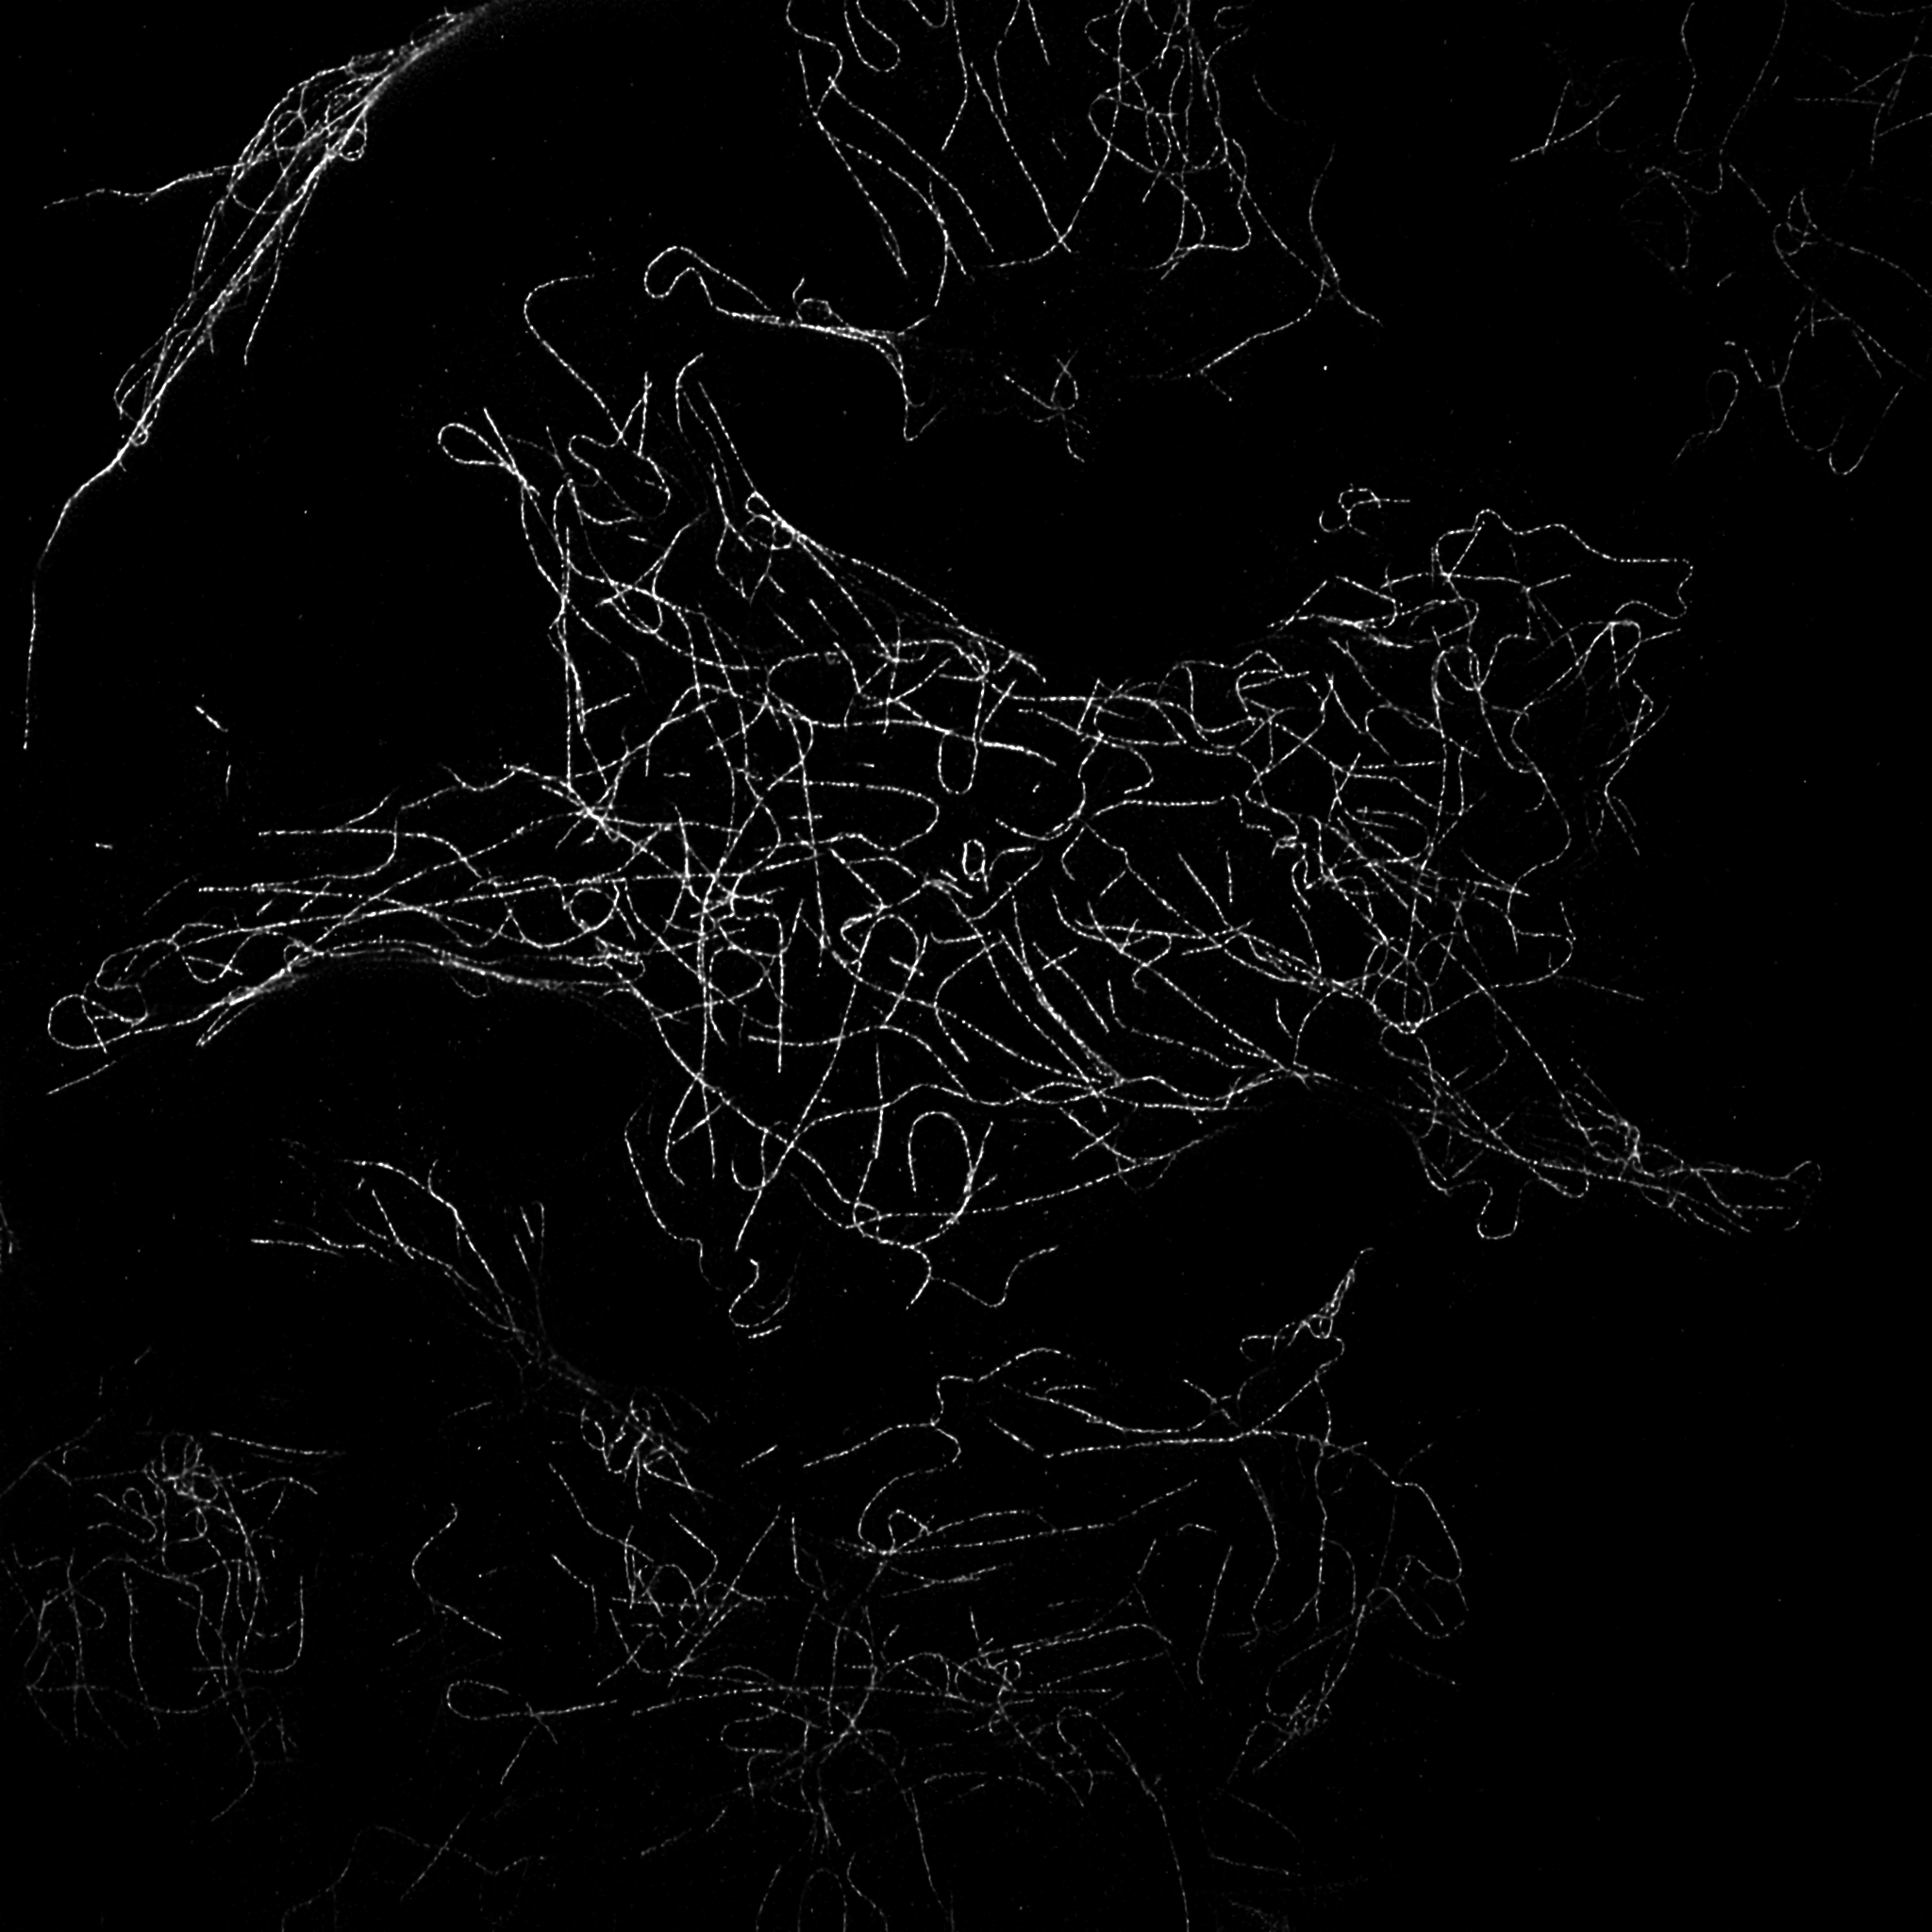
\includegraphics[width=\textwidth]{microtubulos_MAX.png}
\caption{Microtubulos}
\label{fig:Microtubulos}
\end{figure}

\section{Preguntas de Investigaci\'on}
 - Existiendo información a Priori, la que identifica ciertos comportamientos de lo observado (ej: actina no se pega), es posible
 determinar correctamente la cantidad de objetos (estructuras alargadas) y sus caracteristicas con distintos criterios (geometricos comunmente)

\section{Hipótesis}
 - Utilizar enfoque de grafos en base a an\'alisis multi-criterio, lo que permitir\'a obtener mejores resultados

\section{Metodolog\'ia}
%``I always thought something was fundamentally wrong with the universe'' \citep{adams1995hitchhiker}

- Por validaci\'on

\bibliographystyle{plain}
\bibliography{references}
\end{document}
